\documentclass{bmvc2k}

%% Enter your paper number here for the review copy
%\bmvcreviewcopy{??}

\title{A Benchmark on Deep-Learning Convolutional Neural Network for the\\
Representation of Natural Scenes with Large Seasonal Variations}

% Enter the paper's authors in order
% \addauthor{Name}{email/homepage}{INSTITUTION_CODE}
\addauthor{Amandine Gout$^{1,}$}{}{3}
\addauthor{Yann Lifchitz$^{1,}$}{}{3}
\addauthor{Titouan Cottencin$^{1,}$}{}{3}
\addauthor{Quentin Groshens$^{1,}$}{}{3}
\addauthor{Shane Griffith$^{2,3,}$}{}{4}
\addauthor{J\'r\'emy Fix$^{1,}$}{jeremy.fix@centralesupelec.fr}{4}
\addauthor{C\'edric Pradalier$^{2,3,}$}{cedric.pradalier@georgiatech-metz.fr}{4}

% Enter the institutions
% \addinstitution{Name\\Address}
\addinstitution{
 Centrale Supelec,\\
 Metz, France
}
\addinstitution{
    College of Computing, \\
    Georgia Institute of Technology, \\
    Atlanta, USA
}
\addinstitution{
    GeorgiaTech Lorraine, \\
    Metz, France
}
\addinstitution{
    CNRS UMI 2958 GT-CNRS, \\
    Metz, France
}

\runninghead{Pradalier {\em et al.}}{Deep-Learning for Natural Scenes}

% Any macro definitions you would like to include
% These are not defined in the style file, because they don't begin
% with \bmva, so they might conflict with the user's own macros.
% The \bmvaOneDot macro adds a full stop unless there is one in the
% text already.
\def\eg{\emph{e.g}\bmvaOneDot}
\def\Eg{\emph{E.g}\bmvaOneDot}
\def\etal{\emph{et al}\bmvaOneDot}

%------------------------------------------------------------------------- 
% Document starts here
\begin{document}

\maketitle


\begin{abstract}
    This paper focuses on the evaluation of deep convolutional neural networks
    for the analysis of images of natural scenes subjected to large
    seasonal variation as well as significant changes of lighting conditions.
    The context is the development of tools for long-term natural environment
    monitoring with an autonomous mobile robot. 

    We report various experiments conducted on a large dataset consisting of a
    weekly survey of the shore of a small lake over two years using an
    autonomous surface vessel. This dataset is used first in a place
    recognition task framed as a classification problem, then in a pose
    regression task and finally the internal features learnt by the
    network are evaluated for their representation power. 

    All our results are based on the Caffe library and default network
    structures where possible.
\end{abstract}


\section{Introduction}
\label{sec:intro}
Check {\tt bmvc\_guidelines.pdf} for the original text.
- Experimentation of deep learning technique for localization in a natural environment
- Goal: obtaining a seasonal invariant and light invariant representation of natural environment images
- Unique dataset 
- Two different approaches: classification and regression
- Starting point: testing a network (CaffeNet) which performs well on classification task for well known datasets such as ImageNet.

- Classification: ...
- Regression: we try to learn the model that match the image to the GPS coordinates which can allow to identify a place robustly.

\section{Related Works}

%% \begin{itemize}
%%     \item Deep nets for plant recognition \cite{Reyes2015},
%%     \item Deep nets for place recognition \cite{Sunderhauf2015},
%%     \item Change detection across seasons, \cite{Neubert2013}, not based on deep nets
%%     \item the framework of cedric and shane for the lake dataset and image alignements : "Survey Registration For Long-Term Natural Environment Monitoring"
%%     \item Oxford article on regression, \cite{conf/accv/PfisterSCZ14}
%%     \item AlexNet paper with great details on parameter choice, \cite{NIPS2012_4824}
%%     \item OxfordNet, \cite{Simonyan14c}
%%     \item Average faces over American Yearbooks, \cite{ginosar2015century}
%%     \item change detection with CNN \cite{Xie2015}. Mais les images sont pré-alignés et le contexte est du monitoring de surface d'un tunnel
%% \end{itemize}

It is becoming well known that the traditional approach to data association, i.e., point--based feature matching, is unreliable in unstructured environments. It is more applicable the more structured an environment is. Point--based features can be associated well indoors, but special care has to be taken as they are applied in urban environments (e.g., street-view) ~\cite{beall2014, stumm2013}. They lose representational power as the environment changes with night~\cite{nelson2015}, rain~\cite{cord2014}, and shadows~\cite{corke2013}. This means that in some natural environments, like lake shores, point--based feature matching is sporadic even among images from the same survey, and is unreliable between different surveys~\cite{griffith2014iser}. 

The lack of a dominant method for data association in outdoor environments has led to a number of new approaches. All of them function using some form of information beyond the capabilities of point--based features. Image sequence~\cite{milford2012seqslam, cummins2008fab, milford2004, churchill2013, naseer2015}, image patch~\cite{mcmanus2014, Sunderhauf2015a}, and whole image~\cite{arroyo2015, neubert2015superpixel} techniques are becoming increasingly dependable. There are, however, still shortcomings among them. A common limitation is robustness to changes in viewpoint among some approaches based on sequences or whole images. This may not be a factor in monitoring applications, however, since surveys are captured from similar trajectories; the viewpoint and the scale are relatively stable between images (see e.g.,~\cite{milford2014}).

In the recent years, deep neural networks have become very popular methods for solving both classification and regression problems because technical difficulties related to their training have been overcome. In the context of image analysis, convolutional neural networks have been around for several decades because they benefit from inherent regularities in images to constrain the trained architecture and their architecture regularize more general deep neural networks. In the recent years, state of the art performances were achieved with deep convolutional neural networks on various machine learning tasks in the context of computer vision \cite{NIPS2012_4824,Simonyan14c}. Of particular interest for our study, deep convolutional neural networks have been successfully applied to place recognition \cite{Sunderhauf2015b} (a classification task), pose regression \cite{conf/accv/PfisterSCZ14} and viewpoint estimation \cite{Su2015}. Finding the best neural network architecture for solving a given machine learning problem can be very challenging. In this study, we consider the CaffeNet architecture which is an implementation in Caffe\cite{jia2014caffe} of the AlexNet convolutional neural network\cite{NIPS2012_4824}. This network had state of the art classification accuracy on the ImageNet Large Scale Visual Recognition Challenge.




\section{Methodology}

%\subsection{Classification}

One of the major challenge of classification is to properly define classes. We choose to discretize the position into 2,5-meters square. Since the heading is not constant during navigation and can vary a lot without positional change, we also included the orientation of the camera with 10 degrees increments. The objective is to ensure that the images are consistent within each class to limit unnecessary noise during training. 

This representation of the possible position of the robot is very sparse so to improve the efficency of the training, we will limit the number of classes studied. We also need to avoid having a class too strong against the other during the training, our choice is to keep only the classes that have a number of images of at least 50\% of the highest class image count. For our database, this represents around 1000 images per class with 295 classes giving us 300 000 images in total.

We train an implementation of AlexNet on Caffe. We chose Caffe over other deep learning framework because it was easy to use especially for a classification task. AlexNet is a recognized network used for classification. We didn't change the network structure but since we train it from scratch we tuned the number of images used, the size of the mini-batches and the learning rate. We had to find a trade-off between learning time and precision. We used smaller dataset to test the training and to tune those parameters.

--> Include description of the Network (image ?)

The aim was not to obtain a great classification, but to create good features for each class. This means that we are aiming at obtaining convolutional layers that are well formed and rich enough to give a good representation of the image while staying independent of seasonal and local changes.

\subsubsection{Prototypes}
Representations of an image will be found in the network's convolutional layers. As such, we averaged filter responses for every layer over all images in a class. We can thus minimize the impact of variance over the class images (slight heading and position variations). The average of the filter response for one layer of one image gives us a good representation of this image. It can be compared to the prototype of any classes giving us a metric for the similarity of an image to a given class. 


%\subsection{Regression}
The goal of the regression task is to compute the GPS position corresponding to an image of a given place. This image is completely described by the position of the camera and its orientation. Directly using the position and orientation of the camera as labels would have resulted in inhomogeneous labels. Consequently, it was chosen to use a 4-dimension vector. The first two dimensions are the GPS coordinates of the camera and the other two are the coordinates of the projection on the side of the lake in the direction of the view. To ensure convergence the labels were normalized and re-centered. We will refer to the computed scaling factor as \textit{scale} in the following Results section.

For comparison matters the same Network CaffeNet was used for the regression task. Yet some changes were made on the loss layer which previously used the SoftMax function. It was chosen to use the euclidean loss function in this case where the labels are distances. The creation of the dataset is similar to the one performed for the classification.

The implementation was done with Caffe after some modifications so it could deal with real value labels and multi-label regression.


\subsection{Data preprocessing}


<<<<<<< HEAD
The dataset consists in a bit more than 3'000'000 images collected during 80 surveys between the second half of 2013 up to the end of 2015. We consider two experimental setups: a classification task and a regression task. For the classification task, a label is affected to each image based on the pose of the robot. The pose, consisting in the position (from the GPS) and the heading (from the compass) of the robot, is discretized. The position of the robot is discretized into 2.5 meters squares positioned around the lake on a 350 m by 600 m grid centred on a reference point in the center of the lake\todo{how are the blocks positioned ?}. The heading is discretized every 10 degrees. This led to a total of 1'209'600 possible classes.Only a fraction of those possible classes represents images from our dataset and some of the obtained classes were underrepresented. Therefore the dataset was sub-sampled to ensure the balance of the classes. Namely, we kept only the classes with a number of images at least 50\% of the largest class, containing 1750 images. This represents a total of 295 classes with approximately 1'000 images for most classes for a total of 300'000 images on the training set\todo{what is roughly the distribution of the sizes of the classes ? min and max bounds ?} and 5000 images selected randomly for the testing set\todo{how is the dataset split in training and test set ?}. For the regression task, the same set of images was used and the labels were defined from the pose of the robot. One possibility would have been to use the position and heading of the robot as labels but this would imply to define a specific loss taking into account the angular nature of the heading. Although feasible in Caffe, this requires an in-depth modification of the library. Instead, we decided to use an Euclidean loss and therefore defined the labels as a four-component vector with the position of the robot (from GPS) and the position of the point 10 meters away from the robot along the optical axis of the camera\todo{is that true?}. One potential drawback of this approach is that the regression problem becomes more complicated than if we were to predict the position and heading since it requires the regressor to predict a specific location along the heading. However it turns out that despite this constraint, the regressor performed reasonably well (see section~\ref{seg:results-regression}). Finally, in order to ease the definition of the learning rate and to speed up convergence of learning, the labels to be regressed are normalized and centered.
=======
The dataset consists in a bit more than 3'000'000 images collected during 80 surveys between the second half of 2013 up to the end of 2015. We consider two experimental setups : a classification task and a regression task. For the classification task, a label is affected to each image based on the pose of the robot. The pose, consisting in the position (from the GPS) and the heading (from the compass) of the robot, is discretized. The position of the robot is discretized into 2.5 meters squares positioned around the lake on a 350 m by 600 m grid centred on a reference point in the center of the lake \todo{how are the blocks positioned ?}. The heading is discretized as non overlapping angular sectors of 10 degrees. This led to a total of 1'209'600 possible classes.Only a fraction of those possible classes represents images from our dataset and some of the obtained classes were underrepresented. Therefore the dataset was sub-sampled to ensure the balance of the classes. Namely, we kept only the classes with a number of images at least 50\% of the largest class, containing 1750 images. This represents a total of 295 classes with approximately 1'000 images for most classes for a total of 300'000 images on the training set \todo{what is roughly the distribution of the sizes of the classes ? min and max bounds ?} and 5000 images selected randomly for the testing set\todo{how is the dataset split in training and test set ?}. For the regression task, the same set of images was used and the labels were defined from the pose of the robot. One possibility would have been to use the position and heading of the robot as labels but this would imply to define a specific loss taking into account the angular nature of the heading. We rather used an Euclidean loss and therefore defined the labels as a fourth component vector with the position of the robot (from the GPS) and the position of the point 10 meters away from the robot along the optical axis of the camera\todo{is that true?}. One potential drawback of this approach is that the regression problem becomes more complicated than if we were to predict the position and heading since it requires the regressor to predict a specific location along the heading. However it turns out that despite this constraint, the regressor performed reasonably well. Finally, in order to ease the definition of the learning rate and to speed up convergence of learning, the labels to be regressed are normalized and centered.
>>>>>>> da88e1a0cef50cd233a31ccebc38291a16a7514d


\subsection{Convolutional neural network architecture and training}

In this study, we used the AlexNet convolutional neural architecture \cite{NIPS2012_4824} trained in Caffe \cite{jia2014caffe}. The network consists in five convolution layers, five pooling layers, seven rectified linear unit layers, two normalisation layers and three fully connected layers\todo{is it true?}. Minor modifications were required to train successfully the AlexNet network. For the classification task, the size of the mini-batches is decreased to 32 samples and learning rate was decreased at a regular rate 10 times throughout training. \todo{how is it changed?}. For the classification task, the output layer of the fully connected part of the architecture uses a softmax transfer function to get a probability distribution over the labels and the loss is the cross-entropy classification loss. For the regression task, a linear output transfer function is considered and the loss is the Euclidean loss. Experimentally, it was required to consider a lower learning rate than AlexNet which otherwise lead to a divergent loss. As we shall see in the result section, several strategies for setting the learning rate are considered. For both the regression and classification problems, the architecture is trained with the default CaffeNet settings, namely stochastic gradient descent\todo{what is the algorithm used?}, a momentum set to 0.9 and a weight decay to 0.0005.


\subsection{Extracting season invariant representations}

Being able to classify an image as belonging to one part of the lake with its viewpoint or to regress from it the pose of the boat is of interest by themselves. However, one of the objectives of the study was also to extract season invariant representations in order to detect the changes of the lake shore. This part of the study was done only from the network trained in the classification task. For every class of the selected dataset, a prototypical image was computing by averaging all the filter responses, at a given depth of the network, of all the images belonging to the considered class. A query image is then propagated through the network up to the depth where the prototypes have been computed, the responses of all the filters at that depth are then averaged and this representation is compared to the computed prototypes. The quality of the computed prototypical images is then assessed from the cosine similarity between the representation of the query image and the prototypes; labelling a new image is then performed by picking the class whose prototype has the largest similarity with the averaged representation of an image.


\section{Dataset and Experimental Setup}
As mentioned earlier, this paper based its evaluation of CNN for natural
environment on a particular dataset we have been creating since August 2013.
Since then, every 8 to 15 days, we operate an autonomous surface vessel
(Kingfisher from Clearpath Robotics, see fig.~\ref{fig:kingfisher}) around a small lake next to our campus.
This lake is 400m long by 200m wide, with a small island and a total perimeter
of 1km. Its shores are covered with trees, from small bushes to tall full-grown
trees, some at the water line, others further away, grass areas are mixed
with the shrubberies and a small scenic trail runs around the lake. Some of the
places (as in fig.~\ref{fig:dataset-hard}) have office buildings in the
background. 
\begin{figure}[htb]
    \centering
    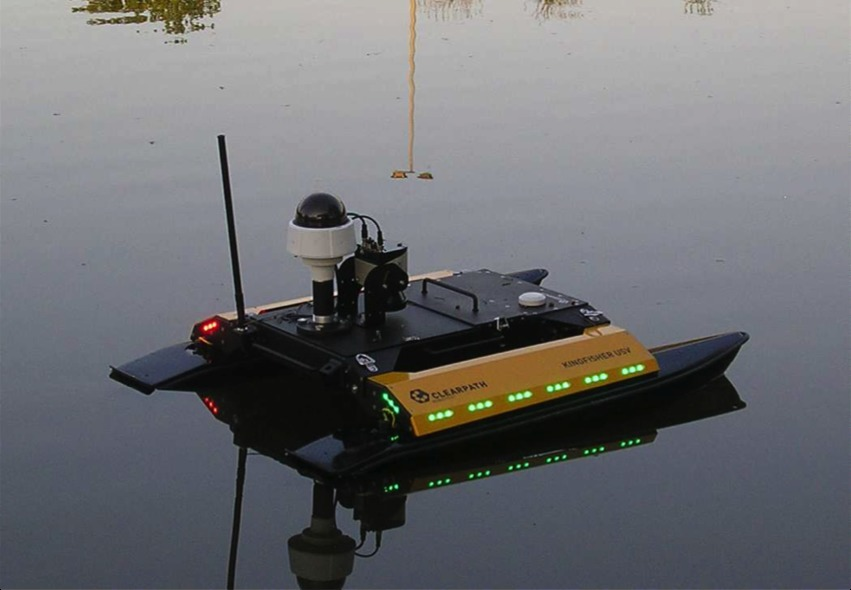
\includegraphics[width=0.4\textwidth]{images/kingfisher}
    \caption{The Kingfisher on a very smooth lake. The pan-tilt camera is
        housed in the white dome at the back of the boat, just behind the laser
    scanner used for navigation.}
    \label{fig:kingfisher}
\end{figure}

Every survey we collect contains images acquired by a pan-tilt surveillance
camera ($704\times480$ pixels) at 10Hz with a slight JPEG compression. The boat
runs autonomously at a constant distance of 10m to the shore (lattice-type
local planner) and at a bit less than 1km/h. This means that a survey is a
collection of close to 40'000 images, acquired with the camera pointing to the
port or starboard side of the boat (i.e. $\pm90^o$ from the direction of
travel). In addition to the images, we record all the boat sensor data:
position from GPS, heading from compass, pitch and roll angle from IMU although
they can be neglected and proximetry from the laser range finder (not used
beyond the on-board controller in this study). 

In this study, we are considering 80 surveys from the second half of 2013 up to
the end of 2015. This corresponds to potentially a bit more than 3'000'000
images collected over 80km of autonomous navigation. 

The particularity of our dataset is that most of our images depicts natural
scenes combining some water, trees and shrubberies at various distances,
sometimes grass areas and/or far-away buildings, and sky. All of these elements
are challenging for computer vision: the lake surface acts as a somewhat
deformable mirror, sometimes very smooth and reflective and at other times not
reflective at all due to wavelets. Additionally, flooding events means that the
water line can move by up to 1m in some surveys. Trees are challenging for
three reasons, first these ones do not always have leaves, second they are
fractal self-similar structures, and last they are 3D semi-transparent
structures whose appearance is very sensitive to view point, especially in
winter. Finally, the sky varies with the weather and the sun position. Because
we run the boat on the perimeter of the lake at different times of the day and
as long as it is not raining (to avoid water drops on the camera dome), our
images are also sometimes affected by sun-glares or very challenging dynamic
range requirements. 

% Dataset:
% - Environmental images from 2013 to 2015
% - Seasonal changes
% - Lighting changes
% - Video frames from camera XXXXX



\section{Results}

\subsection{Classification}
Our best training on the aforementioned dataset was made with 300 000 iterations over mini-batches of size 32 (down from the default 256 for better accuracy), with a learning rate decreasing at a fixed rate ten times during the course of training. The full training took 5 days to finish on a Tesla K20C machine, and attained 70\% accuracy on the test set, on a top-1 classification basis. Such results are satisfactory considering the similarities of natural scene images. It should be noted that classification was not the main goal, but a good classification will intuitively lead to better class representations.

We can thus extract the trained filters responses to see how images as processed by the network. The {\tt conv1} layer will mostly learn edges, namely the skyline and the waterline. {\tt Conv2} detects foliage, and convolutional layers 3 through 5 contain low-level features that are harder to interpret properly. We tested prototype generation on all convolutional layers, as well as the last pooling layer {\tt pool5}, shown in fig.~\ref{prototypes}.

\begin{figure}[htb]
\centering
\begin{tabular}{cc}
    \bmvaHangBox{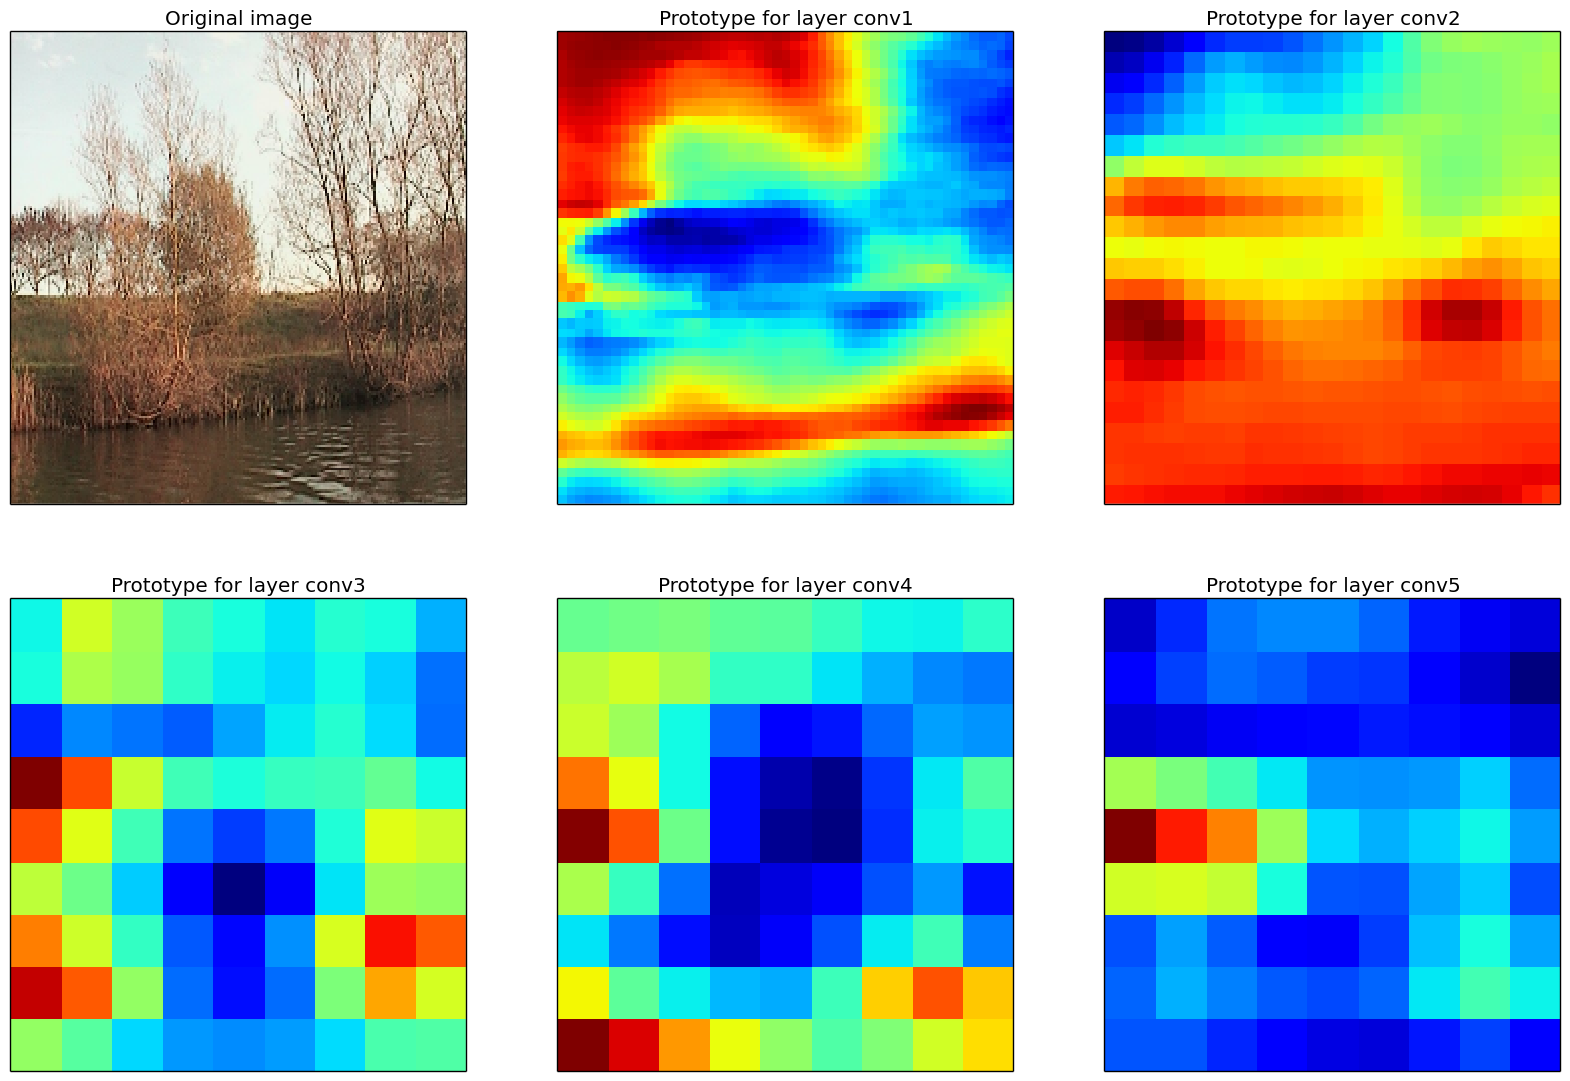
\includegraphics[width=0.8\linewidth]{images/classification/prototypes/avmaskplot7}}\\
\end{tabular}
\caption{Example of prototypes for a given image}
\label{prototypes}
\end{figure}

We generated prototypes for all classes, and tested whether an image can be recognized only using its class prototypes. Testing over a thousand random images and measuring using a cosine distance shows that all layers can be used as suitable descriptors, with distances to the wrong prototypes being indubitably larger than distances to the right prototype on average (see table~\ref{fulltrainvalues}, column 2 and 3 and fig.~\ref{allclft})

\begin{table}[htb]
\centering
\small
\begin{tabular}{|c|c|c||c|c|}
  \hline
  Layer & Overall Ratio & Precision (\%) & Ratio (seen)  & Ratio (unseen) \\
  & (complete dataset) & top-20 & ($1^{st}$ half dataset) & ($2^{nd}$ half dataset) \\
  \hline
  {\tt conv1} & 1.76 & 43.9\% & 1.70 & 1.03 \\ 
  {\tt conv2} & 2.99 & 42.3\% & 0.93 & 0.96 \\ 
  {\tt conv3} & 1.86 & 34.8\% & 1.40 & 0.94 \\ 
  {\tt conv4} & 1.79 & 08.4\% & 1.16 & 1.00 \\ 
  {\tt conv5} & 1.68 & 57.3\% & 1.32 & 0.98 \\ 
  {\tt pool5} & 1.86 & 52.0\% & 1.42 & 0.95 \\ 
  \hline
\end{tabular}
\caption{Ratio of median distance of a random image to the wrong prototypes over median distance to the correct prototype. $2^{nd}$ column refers to the ratio achieved using the complete dataset for training. $3^{rd}$ column give the percentage of successful top-20 classification using the distance to the prototypes of the full dataset. $4^{th}$ column is similar but using only half of the classes. $5^{th}$ column evaluate the generalization performance by evaluating images from the classes not used for training. }
\label{fulltrainvalues}
\end{table}

\begin{figure}[htb]
\centering
\begin{tabular}{ccc}
    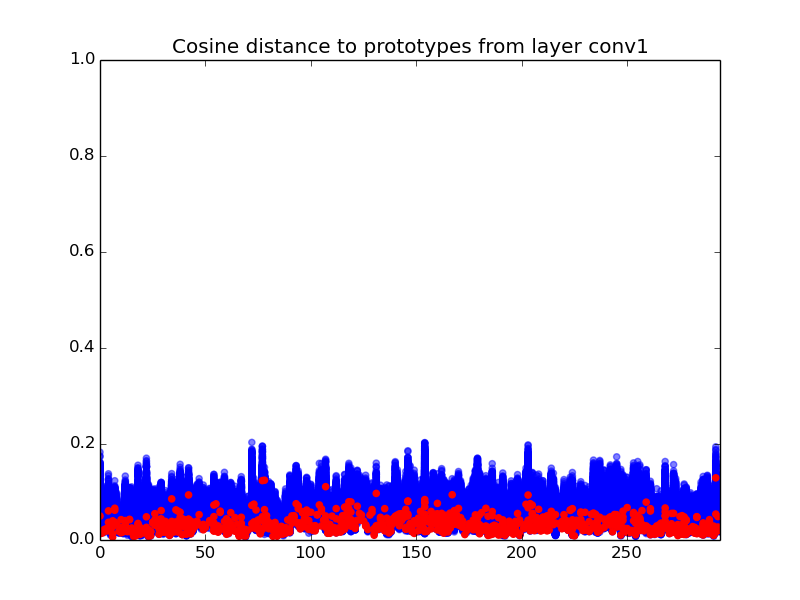
\includegraphics[width=0.3\linewidth]{images/classification/distances/all_classes_full_train/cos_distances_conv1}&
    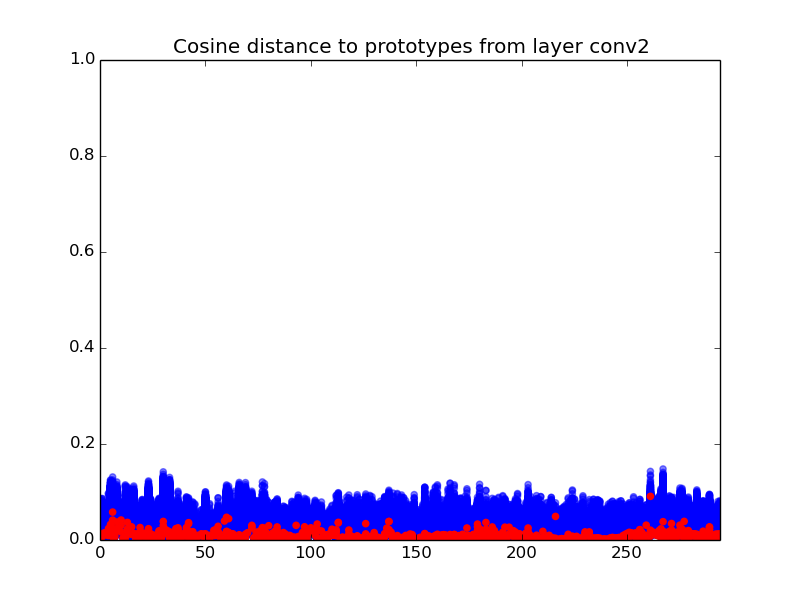
\includegraphics[width=0.3\linewidth]{images/classification/distances/all_classes_full_train/cos_distances_conv2}&
    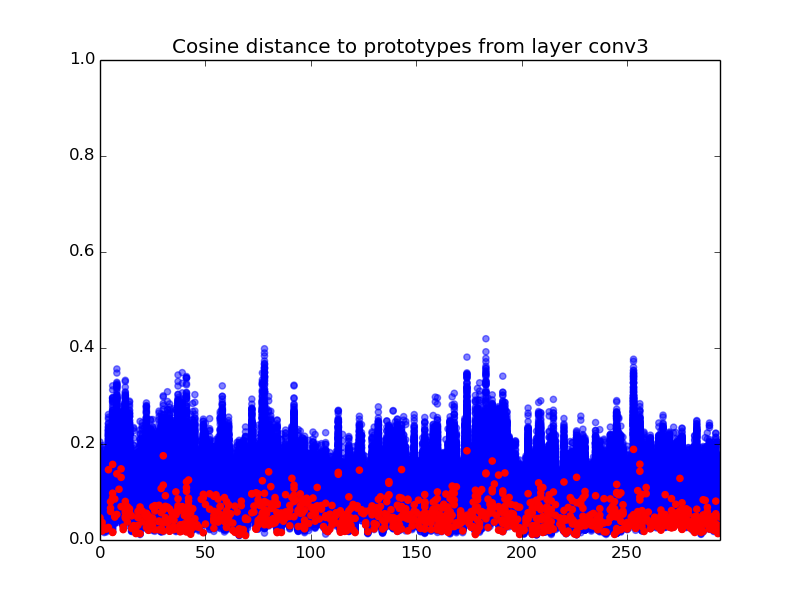
\includegraphics[width=0.3\linewidth]{images/classification/distances/all_classes_full_train/cos_distances_conv3} \\
    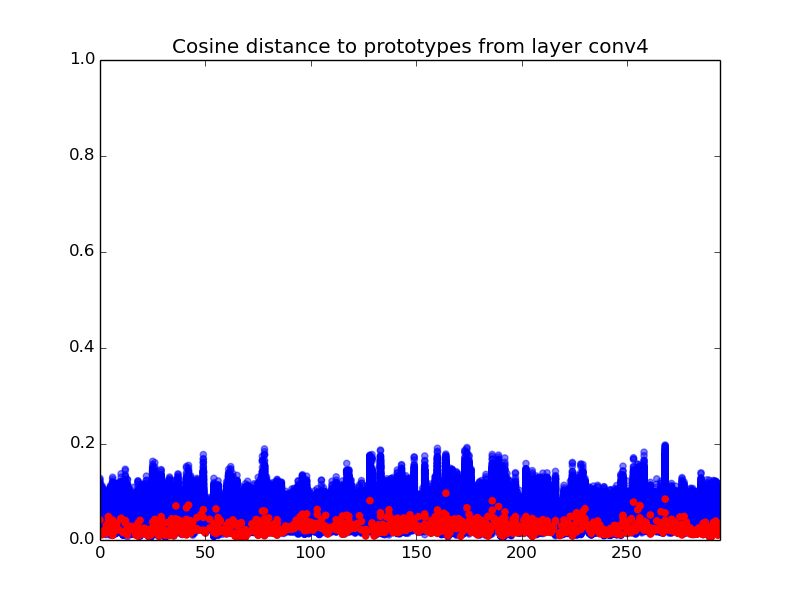
\includegraphics[width=0.3\linewidth]{images/classification/distances/all_classes_full_train/cos_distances_conv4}&
    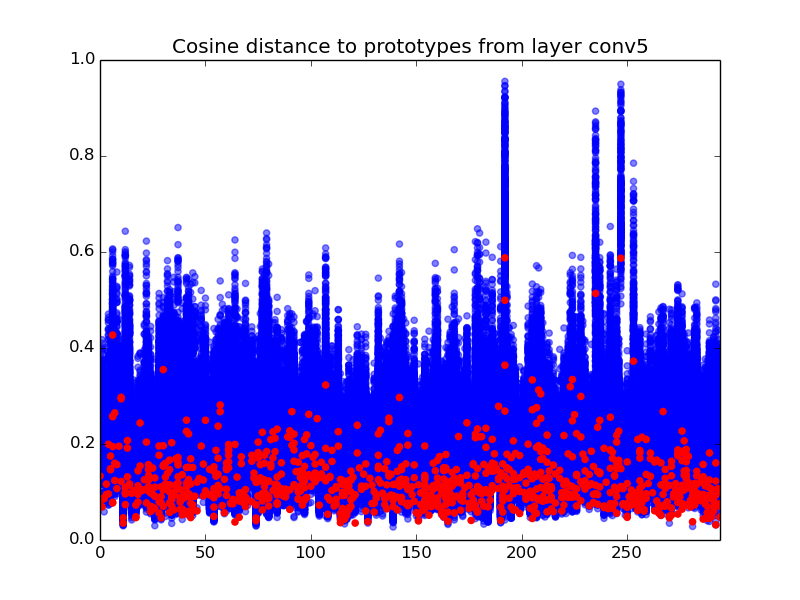
\includegraphics[width=0.3\linewidth]{images/classification/distances/all_classes_full_train/cos_distances_conv5}&
    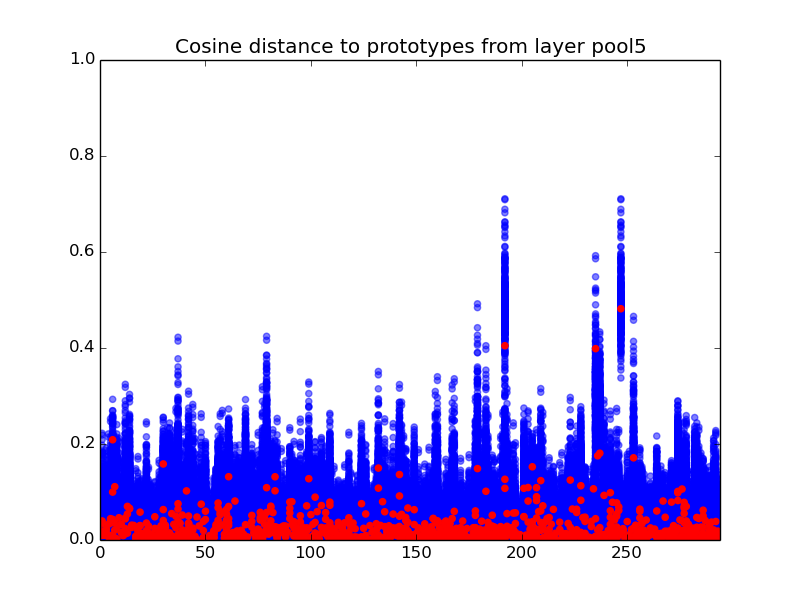
\includegraphics[width=0.3\linewidth]{images/classification/distances/all_classes_full_train/cos_distances_pool5} \\
\end{tabular}
\caption{Red dots represent the distance from a random class image to its class prototype, blue dots are distances to other class prototypes. Graphs show layers conv1 through pool5.}
\label{allclft}
\end{figure}

We also trained the same network on half the classes, to test for generalization capabilities. We wanted to test whether the network learned how to transform an image into its seasonal-invariant representation. %, proved to exist with the full training. % not idea what that means. CP
In the case of the classes observed in the training set, the representation results are analogous to the full dataset. However, the internal features are not discriminative when applied on images from unseen classes (table~\ref{fulltrainvalues}, column 4 and 5). It seems that the network learns how to efficiently discriminate between its known classes, rather than truly learning seasonal variations.

% Merged in table above
% \begin{table}[htb]
% \centering
% \begin{tabular}{|c|c|c|}
%   \hline
%    Layer & Ratio (seen) & Ratio (unseen) \\
%   \hline
%   conv1 & 1.70 & 1.03 \\
%   conv2 & 0.93 & 0.96 \\
%   conv3 & 1.40 & 0.94 \\
%   conv4 & 1.16 & 1.00 \\
%   conv5 & 1.32 & 0.98 \\
%   pool5 & 1.42 & 0.95 \\
%   \hline
% \end{tabular}
% \caption{Ratio of median distances, for seen and unseen classes}
% \label{halftrainvalues}
% \end{table}


\subsection{Regression}
\label{sec:results-regression}
The objective of the regression task is to perform localization with performance comparable to GPS system. The parameters of the training had to be tuned for the network to perform at its best for the regression task.

The layers of the network are initialized using normal distributions. The initialization variances had to be changed from 0.01 to 0.1 for Conv1 and to 0.05 for Conv2, Conv3, Conv4 and Conv5, so that the weights are big enough to propagate information through the network while still ensuring convergence.
The initial learning rate and its evolution policy heavily depends on the loss which is used. For the regression task, very high values and a diverging behaviour were observed with the Euclidean loss at the beginning of the training. The learning rate on the last fully connected layer had to be decreased from 0.01 to 5e-04 to avoid these effects. The learning rate policy was set to the "step" policy from Caffe and it was chosen to decrease the learning rate by half every 25 000 iterations. In our case this corresponds to the number of iterations required to observe the stabilization of the loss after each exponential decrease.

In this context, we tested three different approaches.  The first one consists in training every convolution layer with the same learning rate. The second one consists in fine-tuning the learning rate of the Conv1 layer based on the results given by the first approach. The third one consists in loading the weights of the convolution layers from the classification training. In order to compare our results with those three approaches, we refer to the following loss function :

\begin{equation} 
Loss = \frac{0.5}{scale^{2}}*\sum_{i=1,\ 4}(label_{i}-prediction_{i})^{2}
\end{equation}

The first approach allowed to achieve an average error of 19.3 meters per label as it is shown in fig.~\ref{1apploss}.a. The loss computed on the test dataset is plotted in green and the loss computed on the train dataset is plotted in blue. However after the training, the convolution layers filters did not exhibit any specific features (fig.~\ref{1appfilter}.a). Thus, it appears that the regression was only supported by the fully connected layers. In our case where the goal is to build a seasonal invariant representation of natural scenes this approach did not reach our expectations. 

The second approach led us to push further the difference of behavior between the fully-connected layers and the convolution layers. By increasing the learning rate Conv1 from 0.01 to 0.02, we forced the convolution layers to take part in the regression. This method resulted in being more successful than the previous one. The best average error we achieved was 18.3 meters (fig.~\ref{2apploss}.b). Some natural environment features can be identified in the convolution filters (fig.~\ref{2appfilter}.b).

The last approach used the same learning rate settings as the first approach. It was observed that the convolution weights decreased during the training and ended with a distribution similar to the second approach. The best average error achieved was 20.9 (fig.~\ref{3apploss}.c). However the convolution filters retrieved exhibited different structures than the second approach (fig.~\ref{3appfilter}.c). Based on this result it can be concluded that the convolution weights learned during the classification training could not be reused for the regression task. The weights needed for this task required a smaller variance and the final model presented the worst results among the three approaches. Consequently, learning from normally distributed convolutional gains seems to be more efficient in the case of a regression.

\begin{figure}[htb]
\centering
\begin{tabular}{ccc}
    a) First approach & b) Second approach & c) Third approach \\
    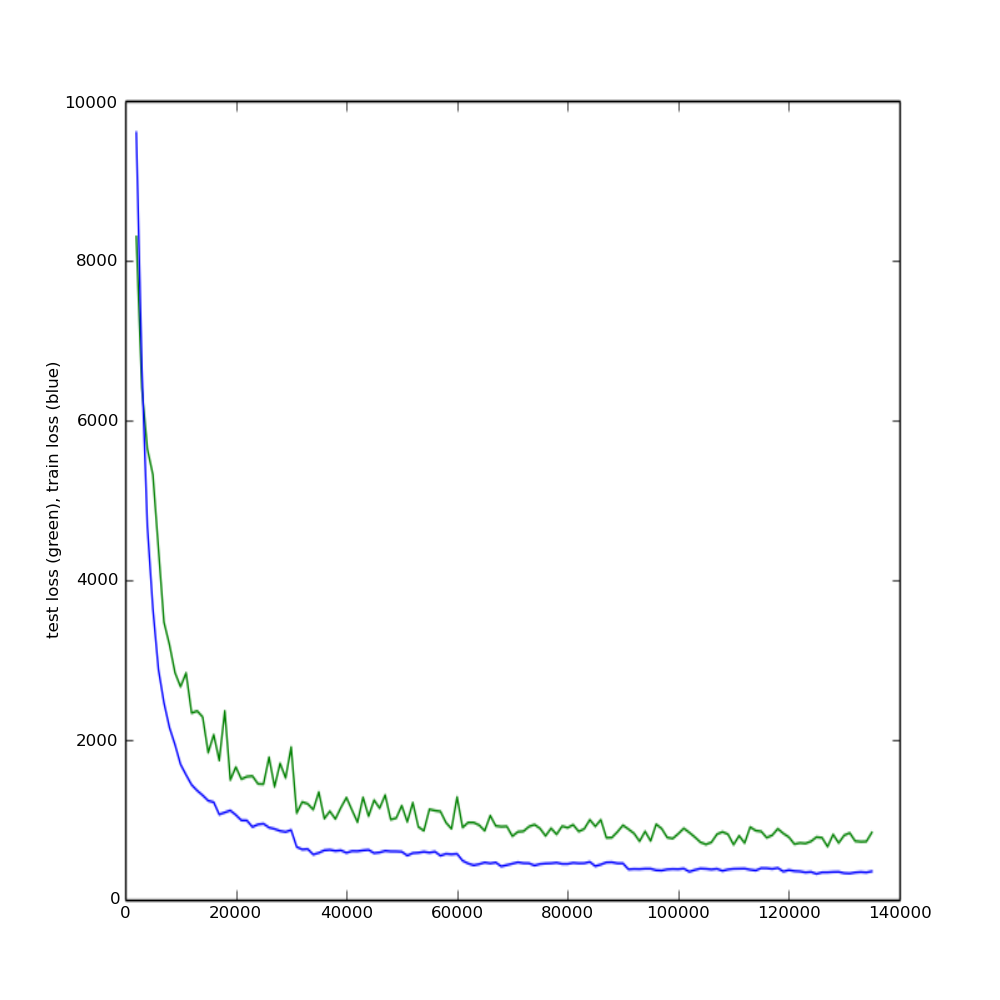
\includegraphics[width=0.3\textwidth]{images/regression/test_loss_26_135000}&
    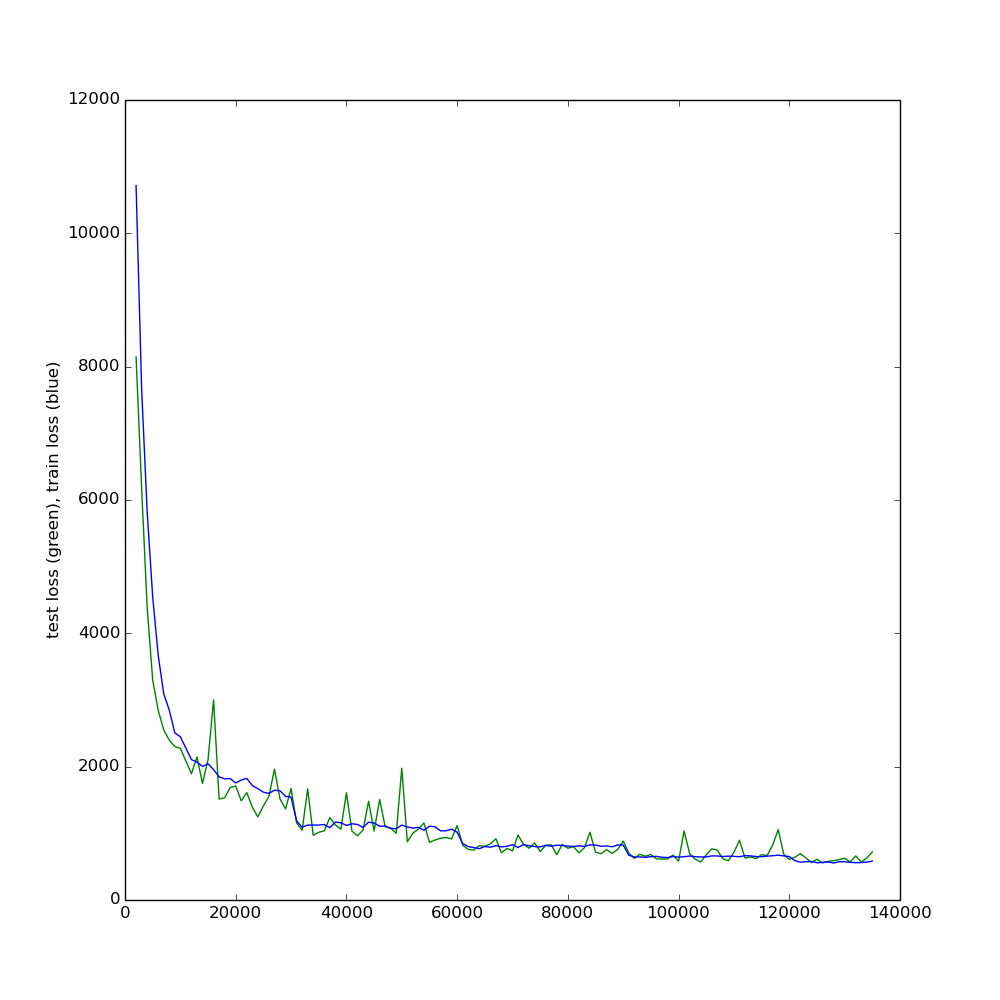
\includegraphics[width=0.3\textwidth]{images/regression/test_loss_37_135000}&
    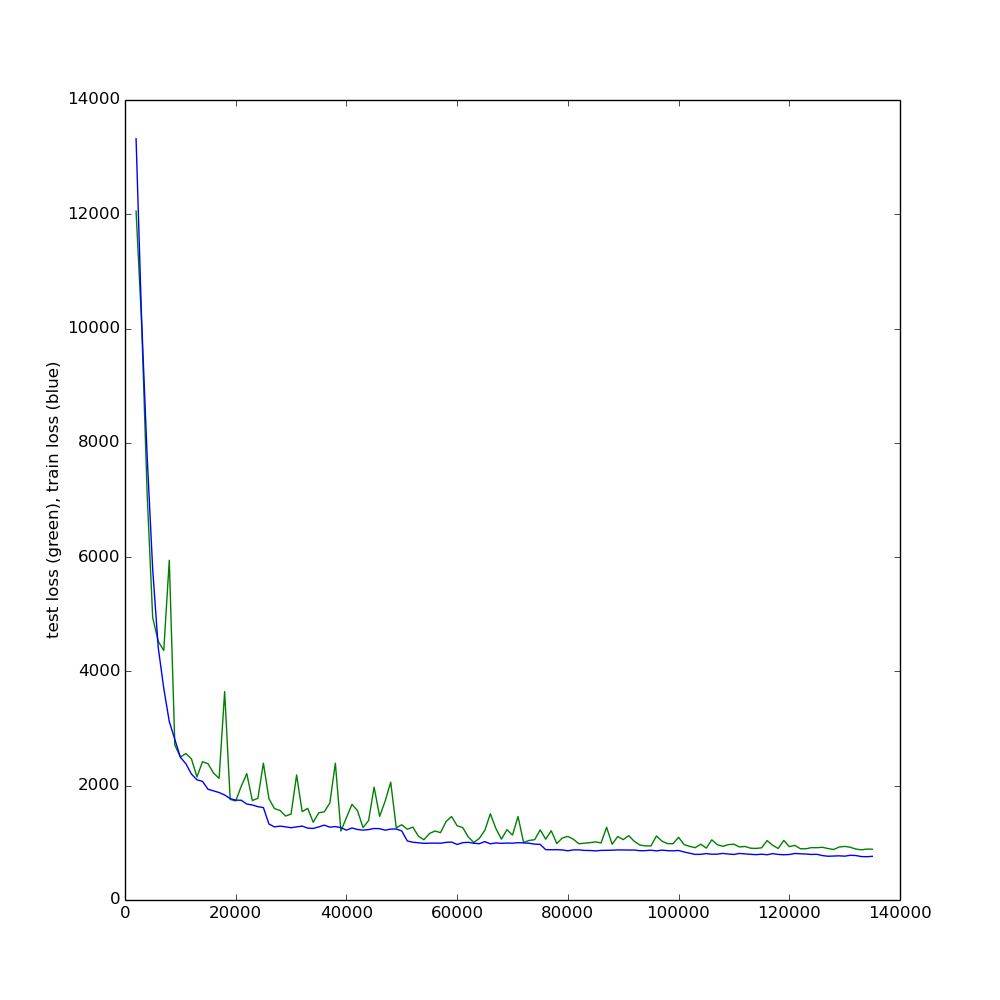
\includegraphics[width=0.3\textwidth]{images/regression/test_loss_30_135000}\\
\end{tabular}
\caption{Loss Function for 135 000 iterations.}
\label{1apploss}
\label{2apploss}
\label{3apploss}
\end{figure}

\begin{figure}[htb]
\centering
\begin{tabular}{ccc}
    a) First approach & b) Second approach & c) Third approach \\
    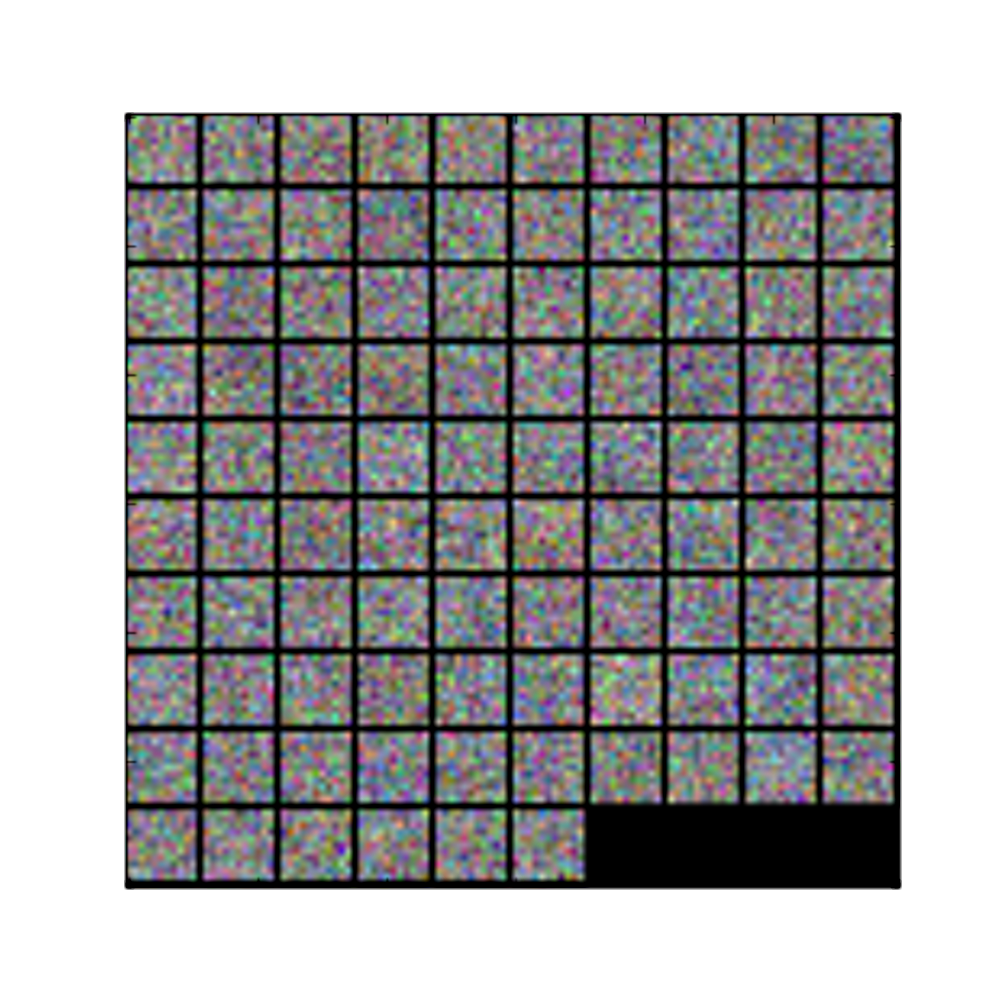
\includegraphics[width=0.3\linewidth]{images/regression/conv1_26_135000}&
    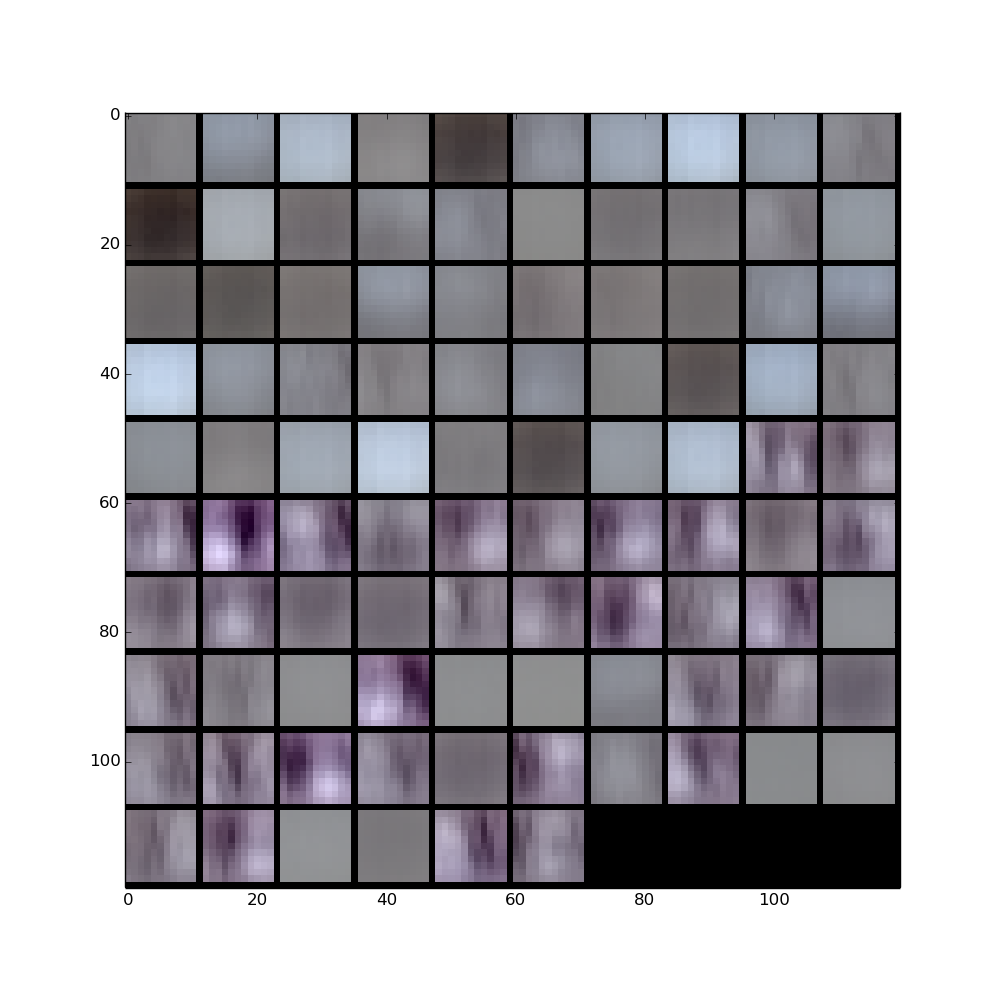
\includegraphics[width=0.3\linewidth]{images/regression/conv1_37_135000}&
    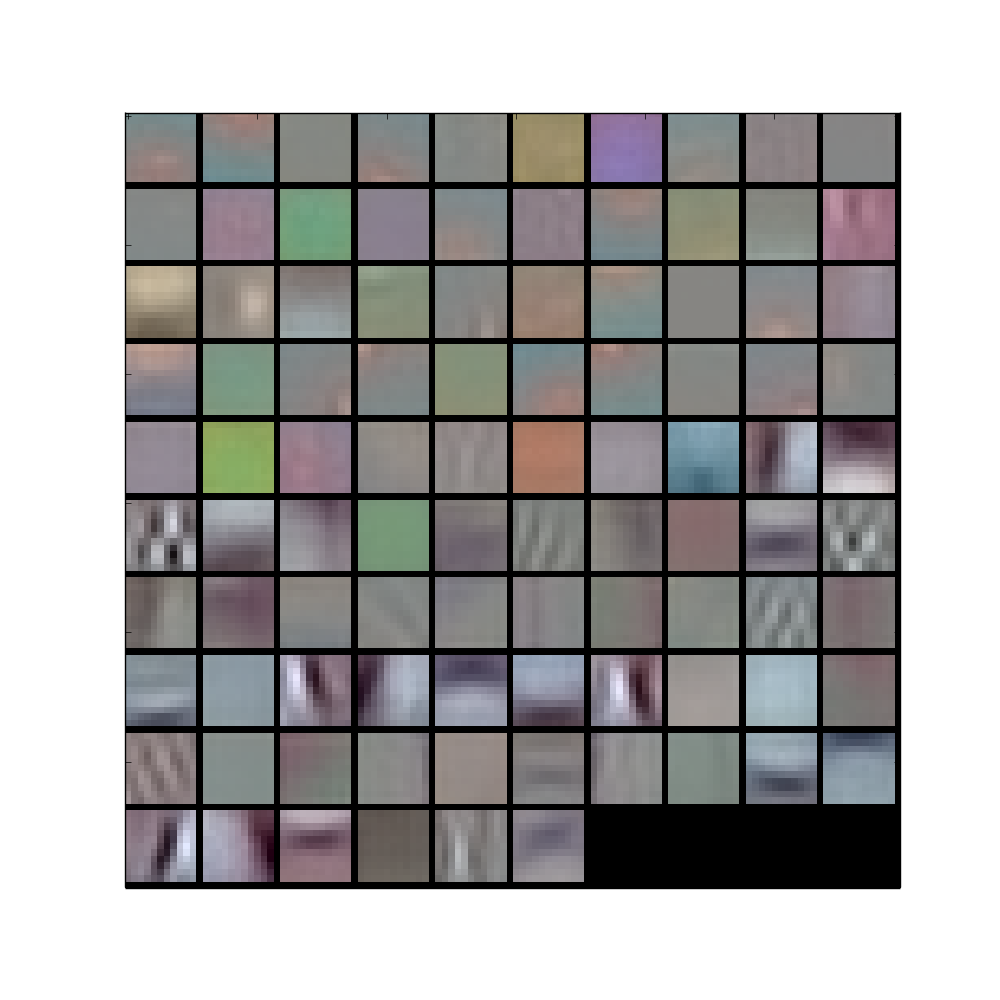
\includegraphics[width=0.3\linewidth]{images/regression/conv1_30_135000}\\
\end{tabular}
\caption{Conv1 filters after 135 000 iterations.}
\label{1appfilter}
\label{2appfilter}
\label{3appfilter}
\end{figure}

The best results regarding the loss values on the train and test datasets were achieved with the second approach. After 148000 iterations, the prediction errors are centered Gaussian-like distributions with a standard deviation of 12.4 meters on X and 20.6 meters on Y. Considering that performing this operation with the human brain is found to be challenging for images from a natural environment, the resulting precision is very acceptable. The labels were displayed to be compared to the predicted positions (fig.~\ref{map}.a and b). The red and green dots represent the original labels and the blue and purple dots represent the predicted labels. The error between X and Y coordinates of the predicted and original labels was also plotted on fig.~\ref{map}.c and was found to be centered on the origin without significant bias.

\begin{figure}[htb]
\centering
\begin{tabular}{p{0.3\textwidth}p{0.3\textwidth}p{0.3\textwidth}}
    %a) Overhead map image with a sample boat path & 
    a) Map of original labels & 
    b) Map of predicted labels&
    c) 2D error of the predicted label position
    \\
    %\bmvaHangBox{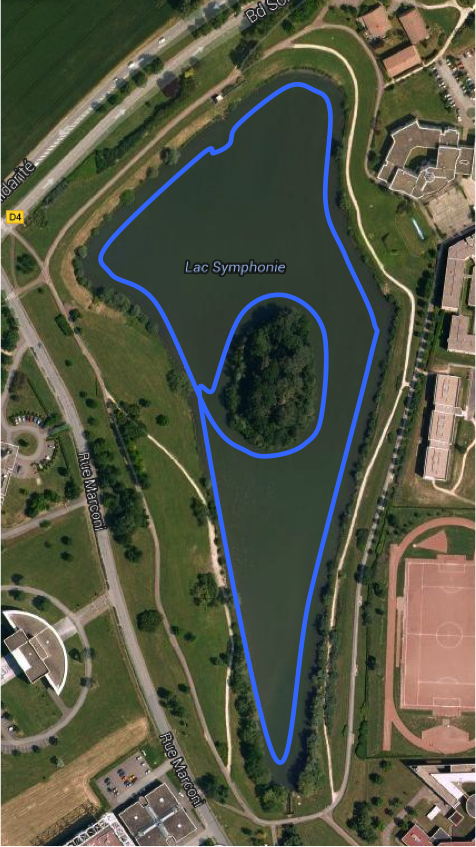
\includegraphics[height=0.4\textwidth]{images/lac}}& 
    \bmvaHangBox{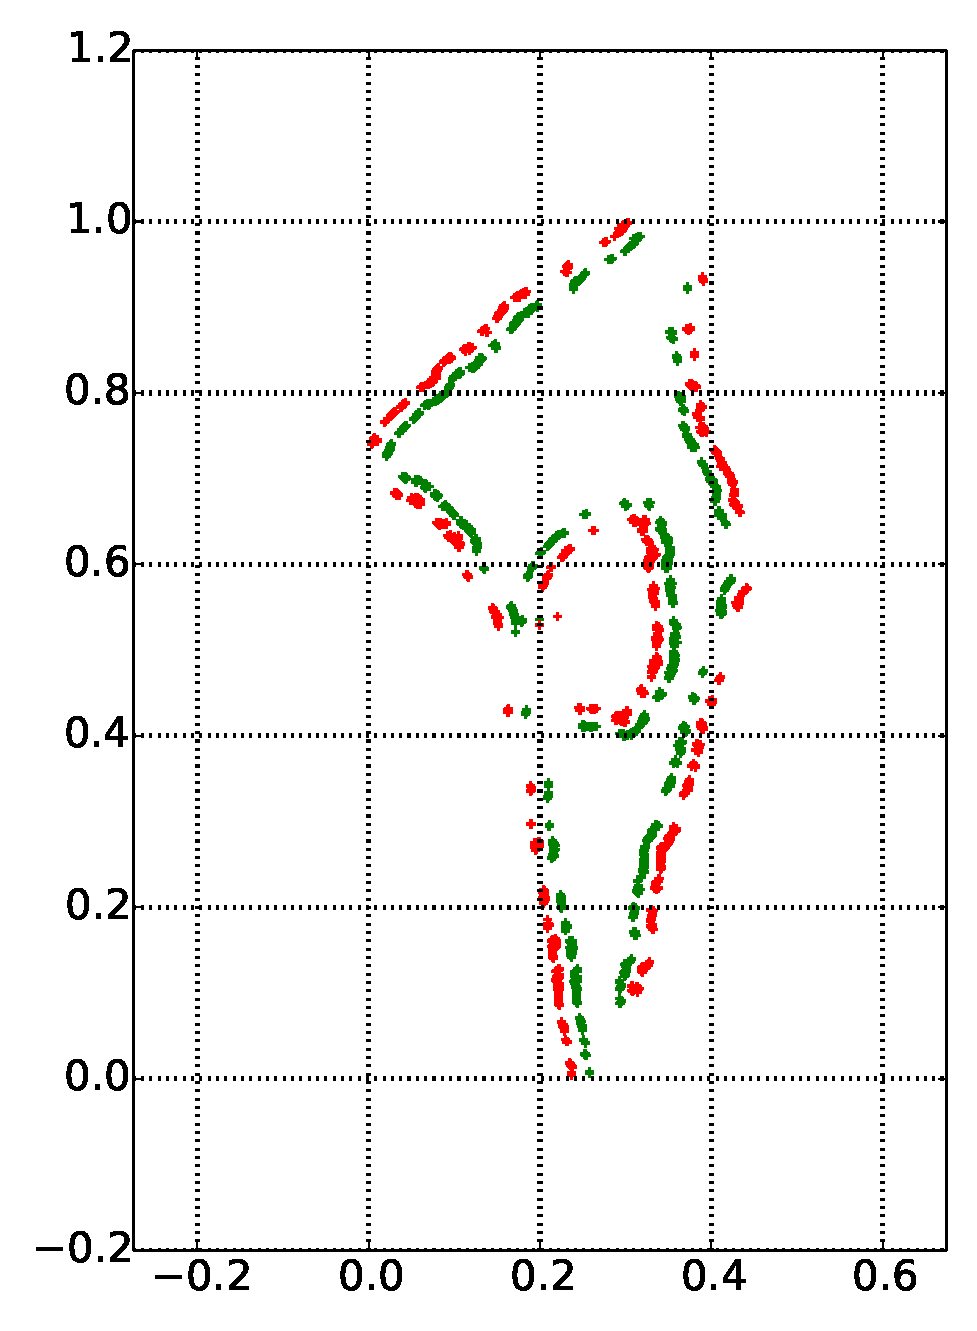
\includegraphics[height=0.4\textwidth]{images/regression/lake_labels_twopoints}} & 
    \bmvaHangBox{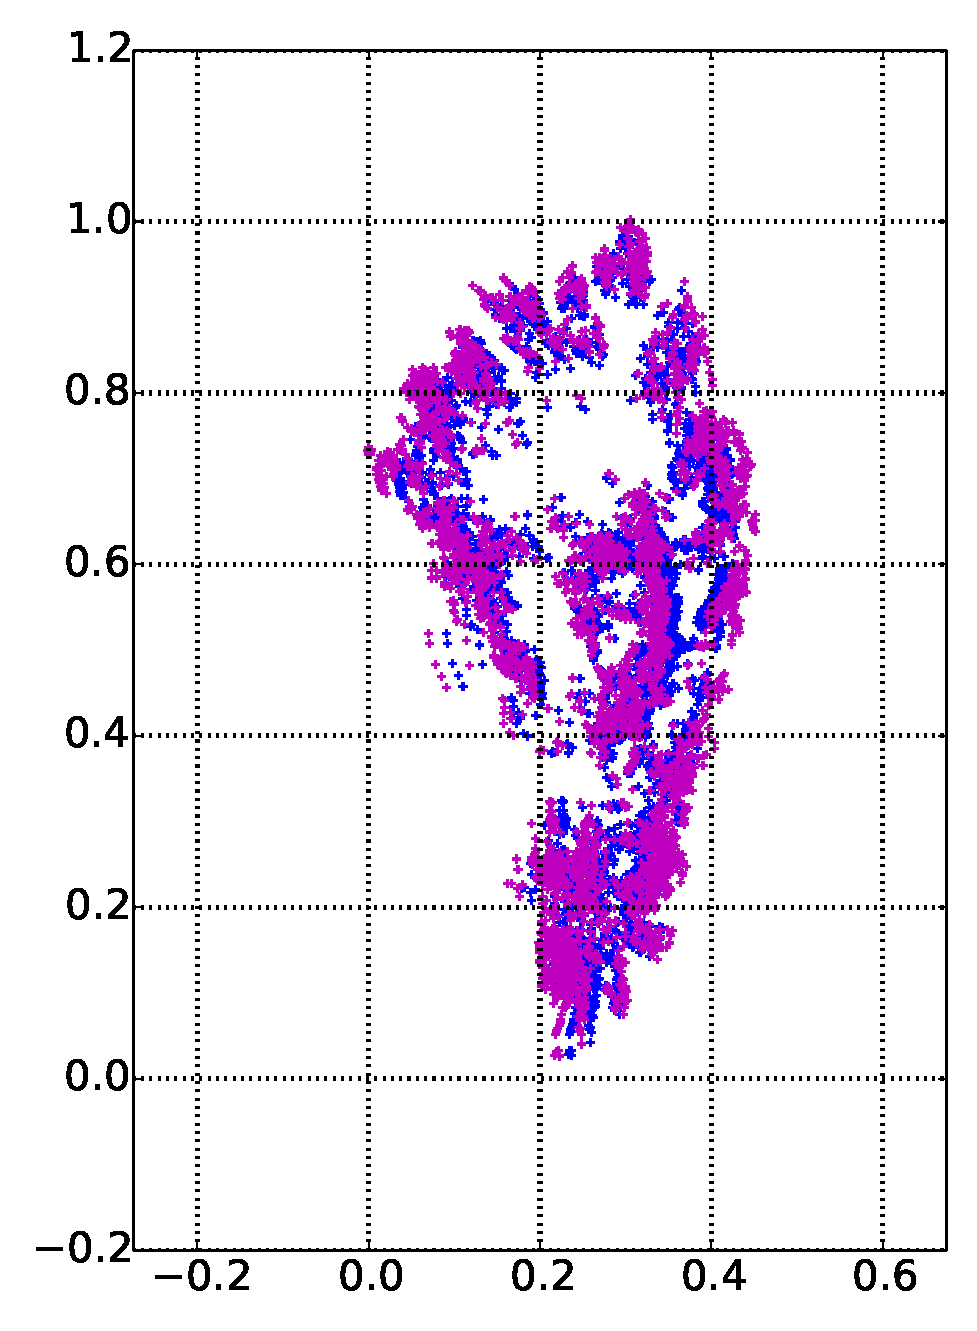
\includegraphics[height=0.4\textwidth]{images/regression/lake_prediction_twopoints}}&
    \bmvaHangBox{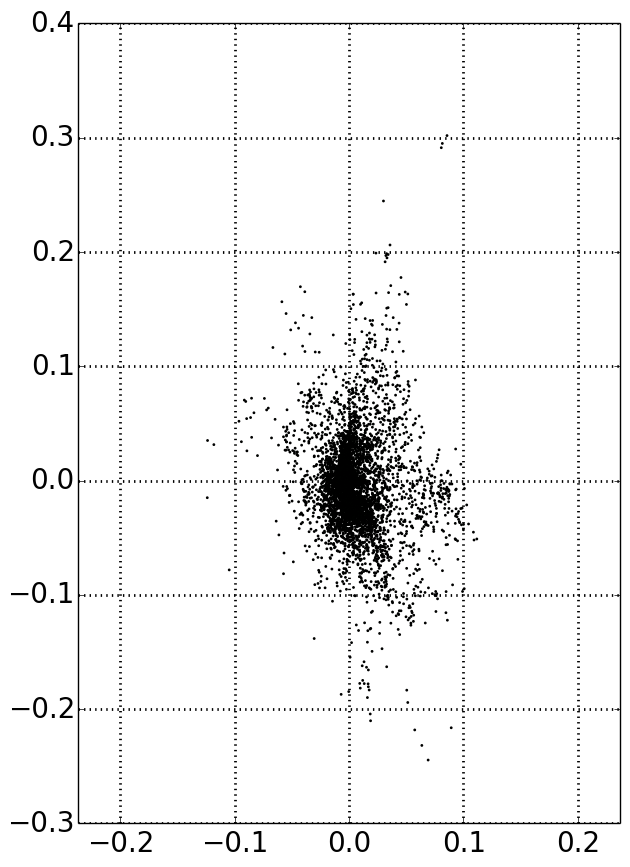
\includegraphics[height=0.4\textwidth]{images/regression/error}}\\
    \\
\end{tabular}
\caption{Map of predicted positions and original labels.}
\label{map}
\label{lake}
\end{figure}

% \begin{figure}[htb]
% \centering
% \begin{tabular}{p{0.3\textwidth}cp{0.3\textwidth}}
%     \bmvaHangBox{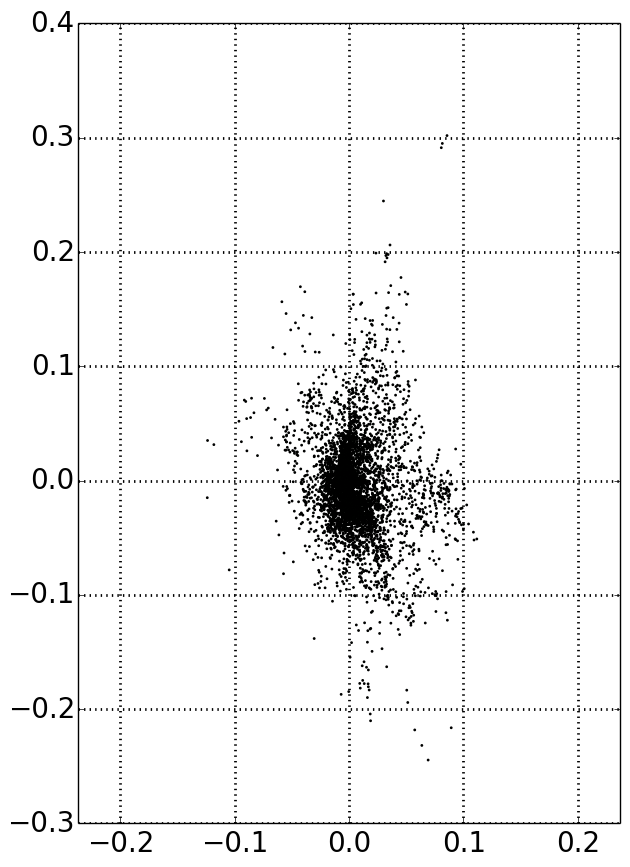
\includegraphics[height=0.3\textwidth]{images/regression/error}}\\
% \end{tabular}
% \caption{Error between X and Y coordinates of predicted and original labels.}
% \label{errormap}
% \end{figure}




\section{Conclusions}
This paper evaluated the performance of convolutional neural network on place
recognition and pose prediction tasks for natural environment under large
seasonal changes, in the context of a long-term autonomous monitoring problem.
To this end, we presented an original dataset consisting in several million
images taken at weekly interval on the shore of a small lake over two years. 

Water and sky appearance inconsistency, as well as the strong seasonal changes
of vegetation and the weather-dependent lighting conditions proved to be
manageable both for the classification task (70\% precision) and for the pose
regression task (20m standard deviation over 1km of shore line). However, it
turned out that using the standard network architecture did not result in
learning generalizable features leading to a season-invariant representation of
the environment. Turning towards more general network architectures as
in~\cite{radford2016} would probably be appropriate but it turned out that
Caffe was too limited to explore this possibility within this study.


%------------------------------------------------------------------------- 

\bibliography{egbib}
\end{document}
